% http://mail.google.com/mail/#search/to%3Akrieger+OR+to%3Adavidahn+OR+(to%3Adavid+AND+to%3Aahn)+OR+from%3Akrieger+OR+from%3Adavidahn/120e6c9667b99ada
\documentclass[letterpaper]{article}
\usepackage{aaai}
\usepackage{graphicx}
\usepackage{times}
\usepackage{helvet}
\usepackage{courier}
\usepackage[usenames]{color}

\pdfinfo{
/Title (FIXME Formatting Instructions for Authors)
/Subject (Proceedings of the AAAI Press Conference)
/Author (AAAI)}
\setcounter{secnumdepth}{0}

% color.sty ... red green blue cyan magenta yellow

\newcommand{\bto}[1]{\textcolor{blue}{\textbf{[#1 --BTO]}}}
\newcommand{\mikeyk}[1]{\textcolor{green}{\textbf{[#1 --mikeyk]}}}

%\newcommand{\codenote}[1]{ \textcolor{cyan}{\textbf{[#1]}} }
\newcommand{\codenote}[1]{}

\newcommand{\link}[1]{\texttt{\small{#1}}}

 \begin{document}
% The file aaai.sty is the style file for AAAI Press 
% proceedings, working notes, and technical reports.
%
\title{TweetMotif: Exploratory Search and Topic Summarization for Twitter}
\author{Brendan O'Connor \\ 
Carnegie Mellon University \\ brenocon@gmail.com
\And
Michel Krieger \\ Meebo, Inc. \\ mikekrieger@gmail.com
\And
David Ahn \\ Microsoft, Inc. \\ daviddahn@gmail.com
}
\maketitle
\begin{abstract}
\begin{quote}
We present TweetMotif, an exploratory search application for Twitter.  Unlike traditional approaches to information retrieval, which present a simple list of messages, TweetMotif groups messages by frequent significant terms --- a result set's subtopics --- which facilitate navigation and drilldown through a faceted search interface.  The topic extraction system is based on syntactic filtering, language modeling, near-duplicate detection, and set cover heuristics.  TweetMotif's subtopic groupings make it easy to obtain both an overview and specific examples of what people are saying; we present examples where it can help deflate rumors, uncover scams, summarize sentiment, and track political protests in real-time.   A demo of TweetMotif, plus its source code, is available at http://tweetmotif.com.
\end{quote}
\end{abstract}

\section{Introduction and Motivation}

%\bto{probably need to cut this intro crap down}

Every day, people around the world broadcast their thoughts to the world as textual messages in various social media.  On Twitter, a recently popular microblogging service, users post millions of very short messages every day.

Organizing and searching through this large corpus is an exciting research problem. Current work has focused on two extremes: (1) showing individual messages, and (2) showing aggregate volume counts.


\begin{figure}[htbp]
\begin{center}
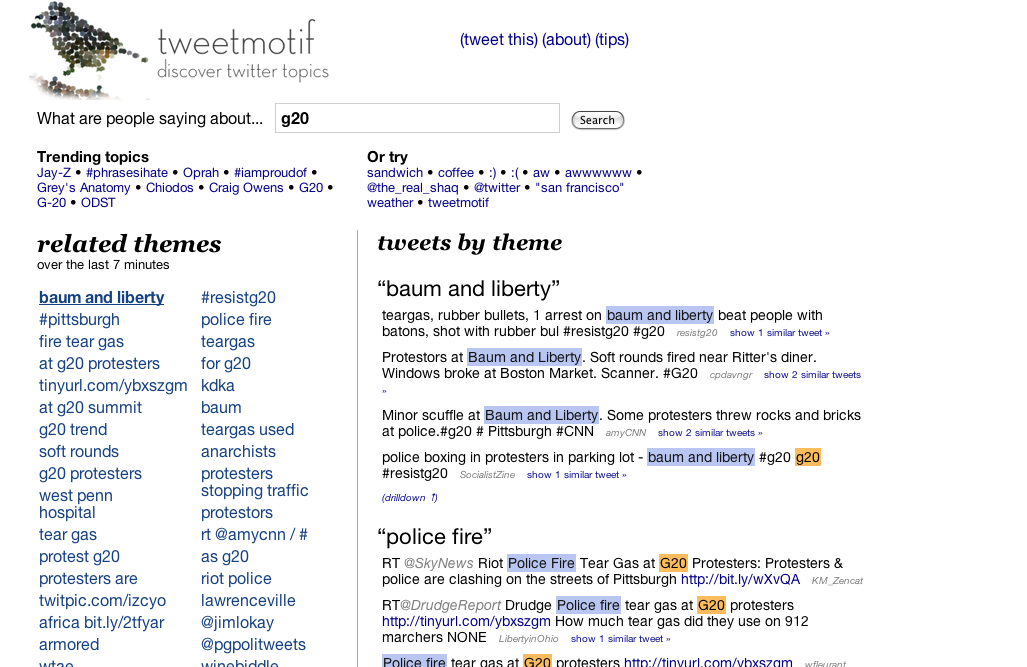
\includegraphics[scale=0.3]{screenshot.png}
\caption{Screenshot of TweetMotif.}
\label{screenshot}
\end{center}
\end{figure}


The most prominent Twitter search systems currently return a flat list of the most recent messages that matched the user query.  This includes Twitter's own search service, \link{search.twitter.com}, as well as recent offerings incorporated into both Google and Microsoft Bing.  This follows the standard approach in web search and traditional information retrieval, where users are often interested in finding a single document that satisfies their information need.  However, characterizing the relevance of microblog messages is an open question; for many information needs, microblog search needs some sort of summarization.

At the other end, there are many efforts that focus on counting the total number of messages matching a term.  The Twitter website prominently features Trending Topics, a list of terms that have been growing in frequency over the last day, week, or month.
%  ... many others  ..   http://trendistic.com/  .. bla bla bla ... 
This is good to help attain a very rough idea of what topics people are talking about, but do little to provide specifics.  Indeed, Twitter's Trending Topics are often so mysterious that a new website was started to collect explanations for what they are (\link{whatthetrend.com}), and at least one Twitter client adds such explanatory blurbs to its user interface (\link{brizzly.com}).

% more stuff found in email and notes
% http://tweetmeme.com  (categories and attempt at a directory)
% http://twemes.com/  (kinda lame, just hashtags)
% http://twitturly.com/ (just url's)
% 
% http://www.launchtweet.com/  a specialized jobs-on-twitter finding site.

%% hmm more criticism.  [[ explain twitter topics ]] is a great google query
% http://blog.hubspot.com/blog/tabid/6307/bid/4694/Why-Twitter-Hashtags-and-Trending-Topics-Are-Useless-to-Marketers.aspx


%%%%%%%%%%%%%%%%%%%% KILL
%Sentiment and opinion analysis approaches ... examples?? ... problematic because sentiment %analysis is a difficult, unsolved task in the field of natural language processing ...

%\mikeyk{How about http://flixpulse.com/ as an example of opinion/sentiment analysis?}

%We believe a different approach is necessary ... want a high-level summary of a corpus of messages, while being able to view individual examples to gain insight ...

%\bto{and a partial screenshot!  but what query? hopefully pick one for a single running example for algorithm exposition.  i'm seriously thinking about \#twitterpornnames, because there's that awesome punchline of the "passwords" topic.  that's the "uncover scams" example i said in the abstract. downside, it's hard to understand on first glance.  also. why not make the screenshot BIG and on the FRONT PAGE!  OUR APPLICATION IS BEAUTIFUL! BOOM!!!}

%\mikeyk{big fan of large first page screenie}

%\bto { oh yeah, and twitterpornnames made it into a dept homeland security warning }

\section{Description of TweetMotif}

Our system, TweetMotif, responds to a user query like a standard search system.  For a query, it retrieves several hundred of the most recent messages that match that query from a simple index; we use the Twitter Search API.

Instead of simply showing the user this entire resultset as a list, TweetMotif extracts a set of topics to group and summarize these messages.  A topic is simultaneously characterized by (1) a textual label, which is a unigram, bigram, or trigram; and (2) a set of messages, whose texts must all contain the label.  The set of topics is chosen to try to satisfy several criteria, which often conflict:

\begin{enumerate}
\item Frequency contrast: Topic label phrases should be frequent in the query subcorpus, but infrequent among general Twitter messages.  This ensures relevance to the query while eliminating overly generic terms.
\item Topic diversity: Topics should be chosen such that their messages and label phrases minimally overlap.  Overlapping topics repetitively fill the same information niche; only one should be used.
%\item Set cover: Topics should be chosen such that their message union includes as much of the query subcorpus as possible, though it is not necessary to i
\item Topic size: A topic that includes too few messages is bad; it is overly specific.
\item Small number of topics: Screen real-estate and concomitant user cognitive load are limited resources.
\end{enumerate}

The goal is to provide the user a concise summary of themes and variation in the query subcorpus, then allow the user to navigate to individual topics to see their associated messages, and allow recursive drilldown.

It could be interesting to formulate these desiderata as a constrained optimization problem,
% (e.g. \bto{cite submodular, constr optim}, 
but in this preliminary work we heuristically fulfill them through several stages of analysis, described as follows.  %\bto{need to slip in excuse that all of tweetmotif was built over a 1 month period.  this may fit well in the Examples section.}

\subsection{Step 1: Tokenization and syntactic filtering}

Tokenization is difficult in the social media domain, and, as is often glossed over in academic natural language processing literature, good tokenization is absolutely crucial for overall system performance.  Standard tokenizers, usually designed for newspapers or biomedical publications, perform poorly.  Our tokenizer correctly handles hashtags, @-replies, abbreviations, times of day, and long strings of punctuation, while preserving emoticons and unicode glyphs (e.g. musical notes) as lexical items.  We made no attempt to handle Asian languages or others that require sophisticated word segmentation, but the tokenizer seems to work well for Spanish and other languages with similar word boundary conventions as English; some queries indeed generate multilingual topic sets.

Unigrams are too narrow a unit of analysis; ideally, we want to extract all phrases and subphrases.  In lieu of developing or adapting a part-of-speech tagger, a prerequisite for standard phrase chunking approaches, we use all unigrams, bigrams, and trigrams (from our fine-grained tokenizations) as candidate topic phrases.  We discard unigrams belonging to a small stopword list of function words, and discard all bigrams and trigrams that cross syntactic boundaries. The rules flag n-grams including certain types of punctuation tokens in certain positions, and ones that end with certain right-binding function words like ``the'' and ``of.''  This simple syntactic filtering greatly improves the coherency of extracted n-grams, though they usually seem worse than the results of a typical phrase chunker.  It often extracts phrases cutting into the named entities and other multiword constructions.

%... hashtags get special treatment: set-like semantics, not allowed to participate in phrases

\subsection{Step 2: Score and filter topic phrase candidates}

\codenote{lang_model.py, ranking.py}
TweetMotif takes a simple language modeling approach to identifying topic phrases.  The language models we use are based on the standard query likelihood retrieval model \cite{manning_introduction_2008}.  Rather than trying to find the documents that best model a set of query terms, though, we are trying to find the phrases that are most distinctive for a tweet result set.  One way of looking for such phrases is to seek out phrases whose probability relative to a language model estimated from a tweet result set is much greater than their probability relative to a language model for tweets in general.  To that end, we score phrases by the likelihood ratio:
\[\frac{Pr(\textrm{ phrase } \ |\ \textrm{ tweet result set })}
{Pr(\textrm{ phrase } \ |\ \textrm{ general tweet corpus })}
\]

Note that we do not try to estimate the probability of phrases on the basis of the constituent tokens in the phrase, i.e., we do not estimate n-gram probabilities from statistics on $(n-1)$-grams or anything like that.  Rather, we estimate the probability of unigram phrases directly from unigram counts, the probability of bigram phrases directly from bigram counts, and the probability of trigram phrases directly from trigram counts.  As is usually the case in language modeling, a given phrase does not necessarily occur in a corpus, so phrase probabilities must be estimated with smoothing.  We tried several simple estimation methods, including maximum likelihood estimation and Laplace smoothing, but settled on Lidstone smoothing:
\[ Pr(\textrm{ phrase }\ |\ \textrm{corpus}) = \frac
{ \textrm{phrase count in corpus} + \delta }
{ N + \delta n }
\]
where for a phrase of length $m$, $N$ is the count of all phrase instances of length $m$ in the corpus, $\delta$ is the smoothing parameter, and $n$ is the count of all phrase types of length $m$ in the corpus.  Essentially, there are independent models for unigram, bigram, and trigram phrases.

%Since we were satisfied with Lidstone, we did not try more advanced language models like Good-Turing, Kneser-Ney, etc.
%.. interestingly, hacky MLE beat Lidstone for a while until tweaked syntactic analysis filtering \bto{explain if room}

The background corpus consists of several hundred thousand randomly collected Twitter messages from April 2008, which is admittedly small and limited.
%.. Backgrond corpus .. say size, admit it's tiny ..

It is interesting to compare our approach to TF/IDF for document retrieval, which estimates document relevance by balancing the frequency of query terms against their frequencies in a background corpus.  Note that the average Twitter message is 11 words long, and words rarely occur more than once in a message; thus, the count of a word is virtually the same as the count of messages it occurs in (DF and TF are the same).  If messages are considered documents, the notion of document TF is not very useful.  Our approach is more like TF for one giant document consisting of the concatenation of all query subcorpus messages.  This too is an odd analogy.  In general, we believe the microblog search problem will require creative formulations of cross-message phonemena beyond current paradigms in IR.

\subsection{Step 3: Merge similar topics}

\codenote{ deduper.py }
Every candidate phrase defines a topic, a set of messages that contain that phrase.  Many phrases, however, occur in roughly the same set of messages, thus their topics are repetitive.  This is undesirable, so we seek to merge similar topics.

First, there are easy merges between subsumed n-gram phrases of differing sizes.  Note that each of an n-gram's label-subsumed (n-1)-grams must conversely subsume its message set.  For example, the message set for the bigram topic ``swine flu'' must be a subset or equal to the two unigram topics ``swine'' and ``flu.''  If the ``swine flu'' topic is in fact equal to the ``flu'' topic, then we discard the ``flu'' topic, since ``swine flu'' is strictly better: we can move from ``flu'' to the more descriptively labeled ``swine flu'' without losing any messages.

%\bto{ LOL wish there was a way to incorporate http://xkcd.com/574/ }

But more generally, there are more difficult cases when topics roughly overlap; we should to merge topics if their message sets are sufficiently similar.  We use the Jaccard set similarity metric, which measures the size of the intersection, scaled from 0 to 1.  It has a value of 0\% if there are no shared messages, and is 100\% if all messages are shared; i.e, the topics are identical.  For topic message sets $s_1$ and $s_2$, merge the topics if:

\[ Jacc(s_1,s_2) = \frac{ |s_1 \cap s_2| }{ |s_1 \cup s_2 | } \geq 0.9 
\]
Topic labels are ignored for this analysis.  All pairs of topics are compared, and final topics are connected components of the pairwise $Jacc \geq 0.9$ graph --- i.e., single-link clustering, so topics less than 90\% similar may end up merged.  When several topics are merged, only the intersection of messages is included in the new topic.  There is a label choice problem/opportunity for merged topics: any of the old topics' labels are now legitimate.  Our heuristic solution usually picks longer and higher scoring labels, and sometimes combines short labels into a skip n-gram.

\subsection{Step 4: Group near-duplicate messages}

\codenote{ deduper.py }
When we implemented the basic topic system, a message duplication issue was revealed: the same, or nearly the same, textual message may be repeated many times.  People forward (``retweet'') interesting messages such as jokes and news headlines; 
%\bto{cite the new boyd et al paper?  kinda lame the wrote a whole paper on retweeting} 
and furthermore, a seemingly huge number of bots repeat advertisements, spam, weather reports, news feeds, other people's tweets, songs being played on personalized Internet radio stations, templated messages, etc.  It is a waste of space to always show near-duplicates to the search user; therefore we detect clusters of near-duplicates, display them with a single representative and numeric size, and allow them optinally to be viewed.%  \bto{awkward}

%.. we use metainfo too

The algorithm simply groups messages whose sets of trigrams have a pairwise Jaccard similarity exceeding 65\%.  (Using a trigram message index cuts down on the potentially quadratic runtime.)  This approximates finding a large shared phrase, since usually two messages share several trigrams only when they are overlapping trigrams from a larger shared n-gram.  We experimented with weighting trigrams by their inverse frequency in the general corpus, but this did not seem to improve results.   

This technique seems to reliably find retweets and other forms of repetition; it also naturally groups together spam.


\subsection{Step 5: Finalize topics}

We are now left with a ranked list of topics containing messages in near-duplicate clusters.  After eliminating topics that contain only one near-duplicate cluster, the list is cut off to the top 40 topics, and all messages that did not end up in a topic are put in a catch-all ``more...'' topic.

\section{User interface}

Rather than the flat list of results commonly presented in Web search, we opted for a user interface inspired by faceted search, which has been shown to aid Web search tasks \cite{hearst_findingflow_2002}.
%\mikeyk{cite http://portal.acm.org/citation.cfm?id=567525}. 
This allows users to explore the breadth of related themes that might appear for a given search query.

TweetMotif's main UI is a two-column layout. The left column is a list of themes that are related to the current search term, while the right column presents actual tweets, grouped by theme. As themes are selected on the left column, a sample of tweets for that theme appears at the top of the right column, pushing down (but not removing) tweet results for any previously selected related themes. This allows users to explore and compare multiple related themes at once. 

Color-coding is used to highlight occurrences of the original search term and of the currently selected related theme. The interface purposely focuses on the content of the message, rather than the timestamp or author.

%\mikeyk{ wasn't sure what the language we're using in the paper for themes etc, feel free to %correct as needed }


\section{Examples}

Figure~\ref{screenshot} shows an example of using TweetMotif during the G20 summit meeting in 2009.  Many people were tweeting about the G20 protests in Pittsburgh, and many of the topics capture specific locations (``west penn hospital''), actors (``anarchists,'' ``riot police''), etc.  One of the co-authors used TweetMotif to learn where violent protests were taking place --- ``Baum and Liberty,'' a street intersection, appears as the first topic in the screenshot, and clicking on it reveals reports of protests that were happening there.  But checking again 15 minutes later, a new topic,  ``Baum and Morewood,'' had appeared: the protest had moved down a few blocks.

We have compiled many other examples as suggestions in the TweetMotif interface; it also shows the current Trending Topics as provided by Twitter.

%\section{Implementation Notes}
%
%surprisingly, it's fast enough to be usable, despite several steps with quadratic runtime and %everything in pure python.  caching helps.  waiting on twitter search API is actually a %bottleneck.  should be possible to scale this prototype into a full-fledged application.

\section{Related Work}

%Topic models; LSA, LSI, LDA ... also, k-means-style document clustering.  Clusty [[god is there anything else to cite by now??]].

%it's more like query refinement really.  cites ... scirus.com (by FAST and Elsevier)  ... also the major web search engines all do it, though usually not as faceted browsing interface

%.. on topic and clustering models ... All of these approaches suffer from the topic labeling problem. ..  By contrast, we unify the notions of topics and their labels.  This forces a deterministic relationship between a topic's label and the messages under that topic, which ensures maximum transparency to the user.

In the blog and microblog search domain, much of the work on search has focused on its applications and unique characteristics relative to traditional Web search, though some work focuses on improving the search engine  itself. This work includes research that uses temporal data for clustering \cite{alonso_clustering_2009}, or applies information visualization techniques to aid search \cite{ferreira-twitviz}.

It is interesting to compare TweetMotif to previous work on topic modeling such as Latent Semantic Analysis / Indexing (LSA/LSI) and Dirichlet Topic Models (LDA).  In TweetMotif, unlike these
models, all topic-message relationships and representations are discrete (boolean).  LSA/LSI is a vector topic model and LDA is a probabilistic topic model; TweetMotif's topic criteria might be formulated as a \emph{discrete topic model}.  Since user interfaces usually communicate discrete information --- e.g., lists of representative words, or the set of documents belonging to a topic --- the results of LSA, LDA, or document clustering usually have to be discretized anyways for a user interface.  Directly formulating discrete topic models may be a useful approach for future work in exploratory document collection analysis.  %\bto{or .. ``combinatorial topic model'' was the other term i've been batting around.  both are zero hits on google!}


%The topic and navigation system may be compared to query refinement, which helps a user  or topic models

%Our topic-finding system bears a 


\bibliography{tweetmotif.bib}
\bibliographystyle{aaai}


\end{document}
